\section{The Navigators}
\label{sec:navigators}

%-------------------------
\subsection{Project Manager}
\label{sec:navigators:projectmanager}

%-------------------------
\subsection{Symbol Palette}
\label{sec:navigators:symbolpalette}

\texnicle\ includes a comprehensive symbol browser so you can easily find the
symbol you want. To view the symbol browser, select the symbol browser icon
above the project tree.  Figure \ref{fig:symbolpalette} shows this.

\begin{figure}[htbp]
\centering
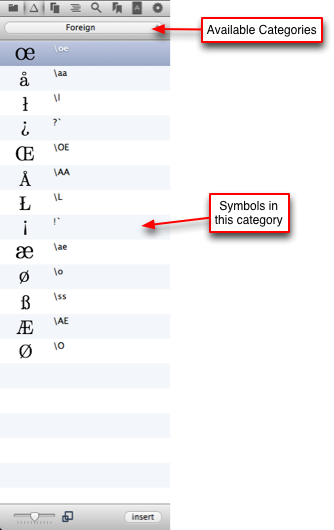
\includegraphics[width=0.4\textwidth]{userguide/images/symbolpalette.png}
\caption{The built-in symbol palette of \texnicle.}
\label{fig:symbolpalette}
\end{figure}

You can also use the keyboard shortcut \texttt{alt-cmd-2}. You will then see the symbol
browser in place of the project tree.

To insert a symbol in to the document currently being edited, select the symbol
you want then click the insert button. Alternatively, you can drag the symbol
in to the text or just double click the symbol to insert it at the current
cursor position.

%-------------------------
\subsection{Code Snippets Library}
\label{sec:navigators:codelibrary}

\texnicle\ has a built-in library where you can store code snippets. You can
organise the snippets into different categories. Some standard categories and
clippings are included to get you started.

To view the clippings library, select the 3rd toolbar icon as shown in Figure
\ref{fig:codelibrary}.

\begin{figure}[htbp]
\centering
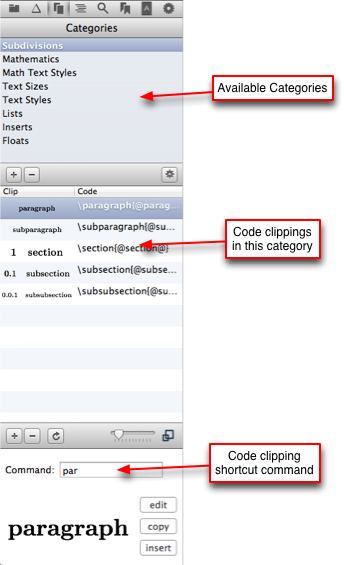
\includegraphics[width=0.4\textwidth]{userguide/images/codelibrary.png}
\caption{The code snippet library of \texnicle.}
\label{fig:codelibrary}
\end{figure}


%-------------------------
\subsection{Document Outline}
\label{sec:navigators:documentoutline}

%-------------------------
\subsection{Project Search}
\label{sec:navigators:projectsearch}

%-------------------------
\subsection{Bookmarks}
\label{sec:navigators:bookmarks}

%-------------------------
\subsection{Spelling}
\label{sec:navigators:spelling}

%-------------------------
\subsection{Project Settings}
\label{sec:navigators:settings}
